\section{Sensitivity Analysis}\label{sec:5-sensitivity-scenario}

In this section, we consider all of the input parameters and how they impact the model's performance and the generated outputs. This sensitivity analysis helps define minimum and maximum values for the input parameters in terms of real-world significance and the model's efficiency/output. 

\subsection{Hard Scattering}

\subsubsection{Variables and Variation Plan}

Here I list the hard scattering variables and the plan for varying their inputs:

\begin{itemize}
\item \textbf{PDFName}: Different PDF sets include different higher order corrections, so it will be good to pick a few of the more popular ones (that aren't too specialized for particular applications) to see how the results are effected.
\item \textbf{ECM}: Higher energy collisions give rise to different cross section values, and hence a different distribution of final events. This will be varied continuously over a moderately wide range. We have to keep in mind, though, that we are attempting to model real world collisions, so we don't want to deviate too much from the $\qty{14}{\TeV}$ used at CERN.
\item \textbf{MinCutoffEnergy}: Like mentioned before, this value is kept moderately above the absolute $\qty{1}{\GeV}$ cutoff to improve efficiency, but we can vary it close down to the level and much higher to gauge how it effects results.
\item \textbf{TransformationEnergy}: This is a purely intermediary calculation variable. It does, however, rely on some of the above input parameters, but itself carries no physical significance. We can vary this widely and see how it effects results.
\end{itemize}

\subsubsection{Results}

\begin{figure}[ht]
  \centering
  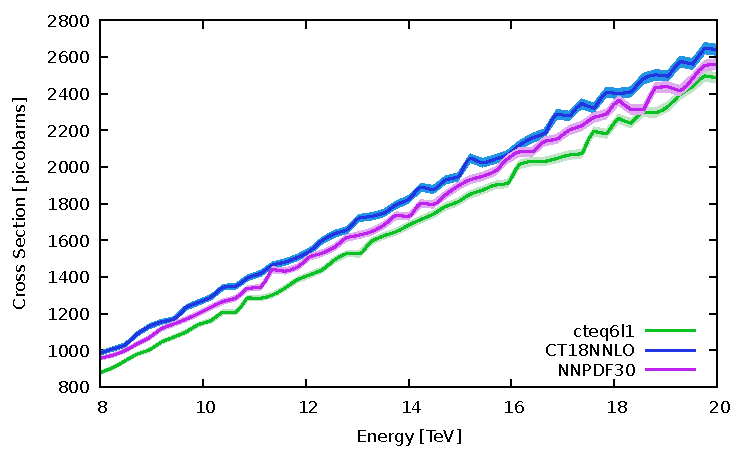
\includegraphics[width=0.7\textwidth]{./res/gfx/xs.pdf}
  \caption{Cross section dependence on center-of-mass energy for the three different candidate PDF sets.}
  \label{fig:ecm}
\end{figure}

Figure~\ref{fig:ecm} contains the curves depicting the dependence of the cross section on the center-of-mass energy, where the shaded region indicates the error. Every other parameter was kept fixed, and we dropped the number of Monte Carlo iterations from one million down a factor of 10 to one hundred thousand (the shading around the lines indicates the error, so one hundred thousand is still more than sufficient for this part). As we expect, the cross section grows monotonically with the ECM. Additionally, we can tell that the most accurate PDF sets increase the total value of the cross section due to the fact that they contain more corrections to the main process. It is interesting how different the curves look, but this is due to vast differences in how different PDF sets are made, so it is not concerning.


\begin{figure}[ht]
  \centering
  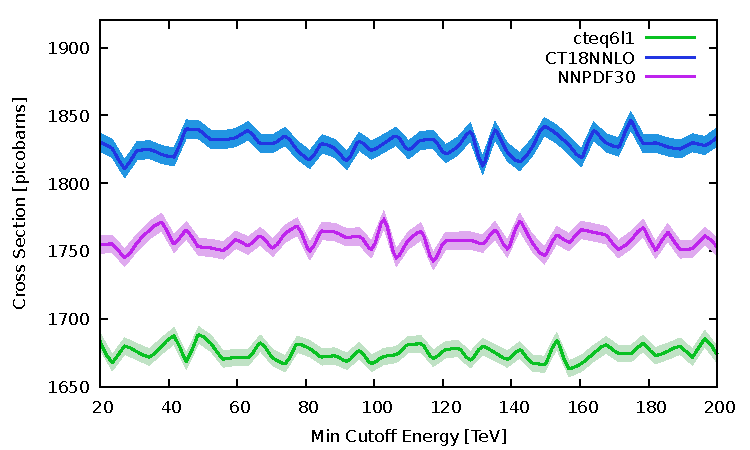
\includegraphics[width=0.45\textwidth]{./res/gfx/cutoff.pdf}
  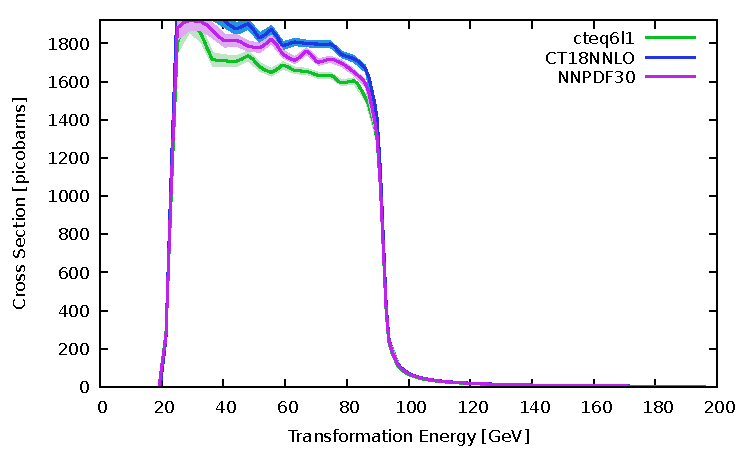
\includegraphics[width=0.45\textwidth]{./res/gfx/transEnergy.pdf} 
  \caption{Cross section dependence on the minimum cutoff energy (left) and transformed mass/width (right) for the three different candidate PDF sets.}
  \label{fig:cutoff-trans}
\end{figure}

Figure~\ref{fig:cutoff-trans} contains similar curves as Fig.~\ref{fig:ecm} but for the minimum cutoff energy and transformation energy. The $E_{\mathrm{CM}}$ was kept fixed at $\qty{14}{\tera\electronvolt}$ and the number of Monte Carlo iterations was kept same. Notably, the cutoff energy seems to not have that much of an impact on the final cross section result as I might have expected, but this may be because of the limited range that I have used. I do know, from my physics knowledge, that the cutoff can only worsen the result. Keeping it within this range, then, is simply a choice the user can make without substantial impact on the final result.

The transformation energy, on the other hand, gives very interesting results. It seems the range of valid results is highly limited between $40$ and $\qty{80}{\GeV}$, and outside this range, there are serious divergences and computational issues. This is not at all what was expected originally, but upon reviewing the places this transformation energy enters, it becomes clear where the issues arise. The center of mass energy for the quark-quark process is denoted $\hat{s}$ and determined by

\begin{equation}
  \hat{s} = M_{\mathrm{tr}}\Gamma_{\mathrm{tr}} \tan\rho + M_{\mathrm{tr}}^2,
\end{equation}

where $M_{\mathrm{tr}} = \Gamma_{\mathrm{tr}} \equiv E_{\mathrm{tr}}$, with $E_{\mathrm{tr}}$ being the transformation energy input parameter\footnote{In principle, one can specify different values for the width/mass, but they always enter the calculation together, so it is not particularly necessary to see how they vary individually.}. The range for $\rho$ is given by

\begin{align}
  \rho_{\mathrm{min}} &= \tan^{-1}\left( \frac{Q_{\mathrm{min}}^2 - M_{\mathrm{tr}}^2}{\Gamma_{\mathrm{tr}}M_{\mathrm{tr}}} \right), \\
  \rho_{\mathrm{min}} &= \tan^{-1}\left( \frac{S - M_{\mathrm{tr}}^2}{\Gamma_{\mathrm{tr}}M_{\mathrm{tr}}} \right),
\end{align}

where this capital, un-hatted $S$ is defined as $E_{\mathrm{CM}}^2$. Evidently, being governed by the $\tan^{-1}$, the two problematic points arise when $E_{\mathrm{tr}} \approx Q_\mathrm{min}$ and $E_{\mathrm{tr}} \approx \sqrt{S}$, which roughly corresponds to the two places the plot diverges. Therefore, it is understood that this value can and should only be changed within this range, and the program should exit upon specifying the parameter to be outside this range.

We next show the dependence of the distributions for the events that were generated after varying the ECM. 

\begin{figure}[ht]
  \centering
  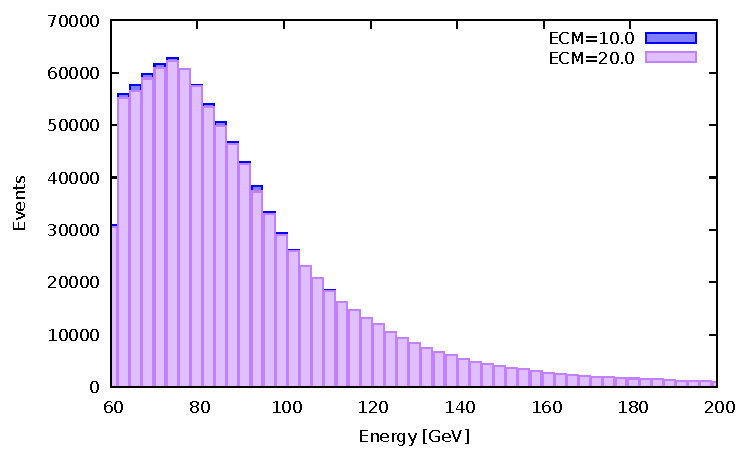
\includegraphics[width=0.7\textwidth]{./res/gfx/Q2.pdf}
  \caption{$Q$ distributions after varying the center of mass energy.}
  \label{fig:q-dist}
\end{figure}

This is done in Figure~\ref{fig:q-dist} for the energy $Q$ of the quark-quark process. It is surprisingly hard to notice, but the lower energy distribution has a sharper peak at a lower energy, while the higher energy distribution has a slightly more spread out peak but is noticeably shifted to the right. The extent to which it is shifted is much smaller than I would have expected, and this is something I was never fully able to figure out. I comment on this again in Section~\ref{sec:7-discussion-conclusion}. However, despite the small difference, it is still absolutely a valid difference, and reflects (at least somewhat) the accurate picture of the physics of the interaction.


\begin{figure}[ht]
  \centering
  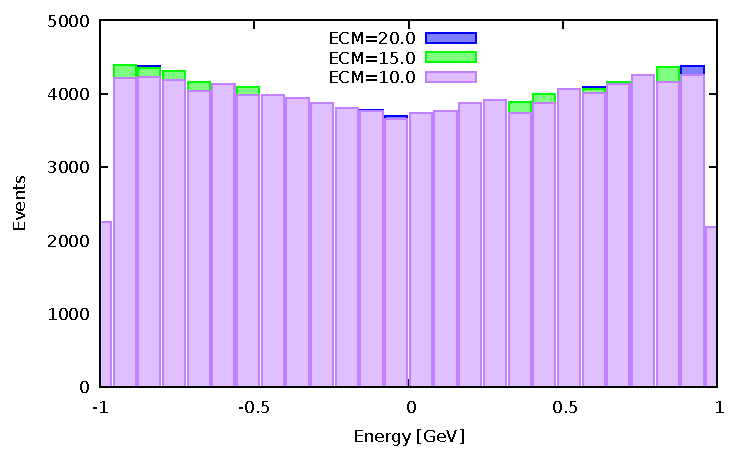
\includegraphics[width=0.45\textwidth]{./res/gfx/cos_theta.pdf}
  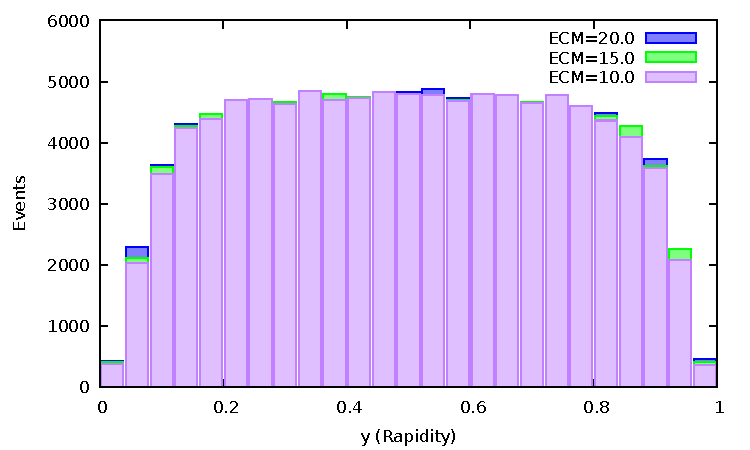
\includegraphics[width=0.45\textwidth]{./res/gfx/y.pdf}
  \caption{$\cos\theta$ and $y$ (rapidity) distributions for varying the $E_{\mathrm{CM}}$.}
  \label{fig:cos-theta-y-dist}
\end{figure}

In Figure~\ref{fig:cos-theta-y-dist} are the distributions for the scattering angle, $\cos\theta$ and the rapidity, $y$, after varying the $E_{\mathrm{CM}}$. These are separated from the main $Q$ distribution since they are symmetric and aren't necessarily related to the absolute value of the $E_{\mathrm{CM}}$, and indeed, this is what we find: there is no particular difference between the distributions at the different energy scales.

\subsection{Parton Showering}

\subsubsection{Parameters and Variance Plan}

Here I list the parton showering variables and the plan for varying their inputs:

\begin{itemize}
\item \textbf{InitialEvolEnergy}: This energy is meant to be on the order of $\qty{1}{\GeV}$, which is the average energy that a hard scattering process will spit a quark out at for an initial $E_{\mathrm{CM}}$ of $\qty{14}{\TeV}$. Therefore, this can be varied a bit above and below, but not too terribly far, since otherwise it would be quite unlikely in a real collision.
\item \textbf{FixedScale}: The other two parton showering variables will both be varied twice, once with this set to Yes and again with it set to No to try and gauge the effects.
\item \textbf{EvolutionEnergyCutoff}: The default of $\qty{~1}{\GeV}$ is the absolute minimum, so it won't be varied any lower. Further, we want to capture as many emissions as possible (as we saw in Section~\ref{sec:4-results}, the $p_T$ distribution, for instance, was peaked at these lower energyes), so it won't be varied much higher.
\end{itemize}


\begin{figure}[ht]
  \centering
  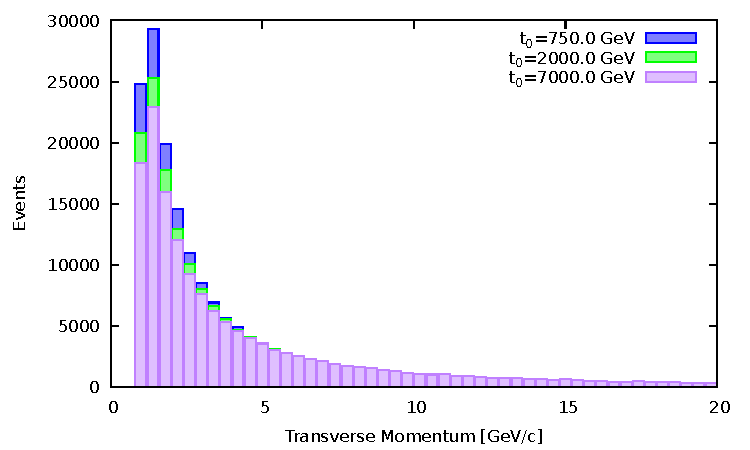
\includegraphics[width=0.45\textwidth]{./res/gfx/pt-fixed2.pdf}
  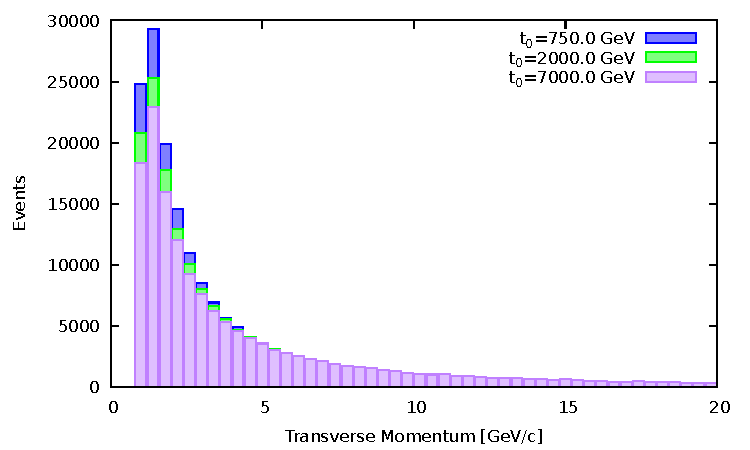
\includegraphics[width=0.45\textwidth]{./res/gfx/pt-variable2.pdf}
  \caption{$p_T$ distributions for the generated parton showering events by varying the initial evolution energy for a fixed scale for the coupling (left) and a variable scale for the coupling (right).}
  \label{fig:pt-dist}
\end{figure}

In Figure~\ref{fig:pt-dist} are two plots containing the output transverse momentum $p_T$ distributions for the generated parton showering events. On the left, the scale for the coupling $\alpha_s$ is kept fixed (and hence its value is also constant), and on the right, it is varied throughout each evolution.

The results here are a little bit more easy to see, and are as expected if we again consider the definition of the Sudakov factor. This factor determined the probability that the quark does \textit{not} emit a gluon from some initial scale $t_0$ to a final scale $t$. This means that for a particular evolution starting at a $t_0$ which is higher compared to another at $t_0'$, it is essentially just as probable for the former evolution to emit a quark at a $t$ which is higher compared to the latter evolution at $t'$. The point is that it is more likely to emit gluons at a higher evolution scale when starting the evolution itself at a higher value (phrasing it this way makes it seem very intuitive, but it helps to have a mathematical grasp).

This is reflected in the plots since we see that the distributions corresponding to higher initial evolution scales are shifted to the right and are a bit more spread out with more events occurring at higher energies, corresponding to the fact that higher $p_T$ events are more likely. Evidently, the model is performing as expected in this regard. Another thing that we notice is that varying the coupling vs. keeping it fixed seems to have very little effect. This is expected: the fixed coupling is chosen to be at the scale of half of the initial evolution scale, meaning that, on average, it \textit{roughly} captures what the variable coupling would capture. Only super minor effects would matter, and those are impossible to tell in the graph. Further, the ``additional effects'' are only NLO effects, not NNLO or N$^3$LO (the order to which corrections to the couplings are known), meaning they are already very small.

\begin{figure}[ht]
  \centering
  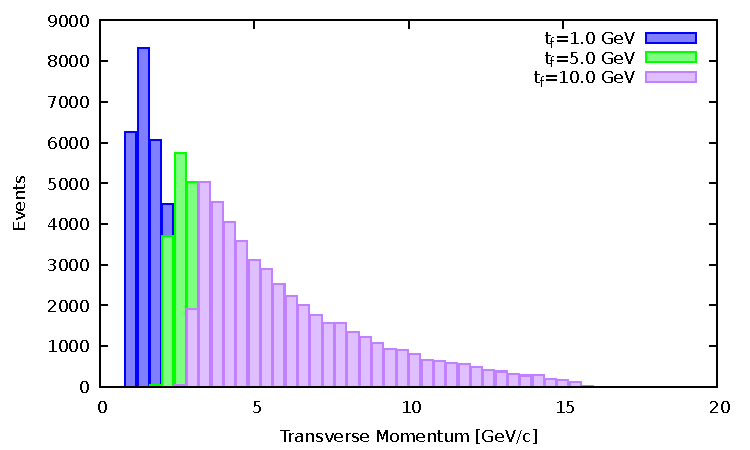
\includegraphics[width=0.45\textwidth]{./res/gfx/pt2-fixed2.pdf}
  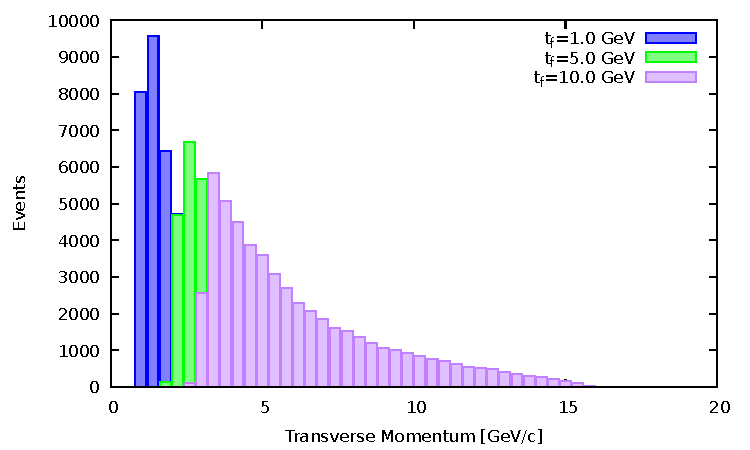
\includegraphics[width=0.45\textwidth]{./res/gfx/pt2-variable2.pdf}
  \caption{$p_T$ distributions for the generated parton showering events by varying the evolution cutoff energy for a fixed scale for the coupling (left) and a variable scale for the coupling (right).}
  \label{fig:pt-dist2}
\end{figure}

In Figure~\ref{fig:pt-dist2}, I have done the same but this time by varying the final cutoff energy. This had the most notable effect of dramatically reducing the number of emissions that were generated by the end for the cases with higher cutoff. Further, the shape of each distribution is essentially identical, which makes sense. This is exactly as expected and shows further that the model works as expected.


\subsection{Scenario Analysis}

From my understanding of scenarios, as they are used in the context of this assignment, I believe that my model is incompatible with them. My reasoning ties back to what has been described about my model's specifics previously. In particular, the nature of my model simply doesn't allow for ``optimistic'' or ``pessimistic'' or any type of scenario at all, because there is nothing necessarily good or bad to expect. The example in the assignment gives things like higher or lower demand in the markets, which have good/bad real-world consequences. My model, on the other hand, is a model of a process in quantum physics. The behavior and mathematics the underpin it very tightly bind the process to behave in only a specific way, a part of which I attempt to capture with my model/simulation.

What I am trying to convey is that there are only two concrete scenarios for my simulation: either I follow the theorems and implement what is known in the current literature and accurately simulate what happens in the real world, or I violate any one of the dozens of theorems and assumptions in place that make modeling/simulating the model possible in the first place. Further, as a model that doesn't necessarily have the same effects directly on the everyday lives of people as traffic models or economical models, it is significantly harder to quantify what is even ``optimistic'' or ``pessimistic'' in the first place. The physics either occurs as expected, or doesn't -- there's nothing else to it.

Therefore, I believe that it is not beneficial (or possible, really, without really stretching some things) to define scenarios and carry out this particular part of the procedure. I feel that, in the previous section, I have done as much as I can in terms of validating how the model performs under the changing of the various input parameters. I have also done my best to tie the changing of the input parameters to their physical interpretation in order to try and match at least some of the requirements of this section.


\subsection{Final Parameter Ranges}

\begin{table}[ht]
  \centering
  \begin{tabular}{|c|c|c|c|c|}
    \hline
    Variable & Default & Min & Max & Notes \\ \hline
    $E_{\mathrm{CM}}$ & $\qty{14}{\TeV}$ & $\qty{-6}{\TeV}$ & $\qty{+6}{\TeV}$ & None \\ \hline
    $E_{\mathrm{min}}$ & $\qty{60}{\GeV}$ & $\qty{-50}{\GeV}$ & $\qty{+440}{\GeV}$ & None \\ \hline
    $E_{\mathrm{tr}}$ & $\qty{60}{\GeV}$ & $\qty{-20}{\GeV}$ & $\qty{+20}{\GeV}$ & Tied to $E_{\mathrm{CM}}$ and $E_{\mathrm{min}}$. \\ \hline
    $t_0$ & $\qty{1000}{\GeV}$ & $\qty{-250}{\GeV}$ & $\qty{+5000}{\GeV}$ & None \\ \hline
    $t_f$ & $\qty{1}{\GeV}$ & $\qty{-0}{\GeV}$ & $\qty{+10}{\GeV}$ & Hard minimum cutoff. \\ \hline
  \end{tabular}
  \caption{Definitive table defining the absolute sensitivities of the possible input parameters.}
  \label{tbl:input-sensitivities}
\end{table}

In Table~\ref{tbl:input-sensitivities} is a definitive list of all the min and max values each input parameter can take. The PDF name and fixed $\alpha_s$ scale are omitted since those are discrete variables, and in principle, any recent PDF can work and either fixed or a variable scale is perfectly valid for the simulation.


%%% Local Variables:
%%% mode: LaTeX
%%% TeX-master: "../../FinalMilestone"
%%% End:
